% !TEX root =  master.tex 
\chapter{Erstellen des Mockups -- Manuel Techert}

\section{Erstellen des ersten Mockups}

Um eine Vorstellung davon zu bekommen, wie unsere Benutzeroberfläche später einmal aussehen soll, wollten wir vorhandene Ideen visualisieren. Dazu benutze ich Sketch, ein Design-Tool für macOS, welches das Gestalten von Oberflächen aller Art ermöglicht.

Zunächst sollen zwei verschiedene Situationen visualisiert werden - Das Log-in Fenster und das Spielefenster.

Bei dem Log-In Fenster sollen zwei Eingabefenster realisiert werden. Da das Spiel nicht lokal, sondern über mehrere Computer gespielt werden kann, habe ich eine einfache Anmeldemaske mit zwei rechteckigen Feldern mit den Eingaben Benutzername und Passwort erstellt.
Nach erfolgreichem Anmelden auf dieser Maske, soll der Benutzer zum eigentlichen Spiel weitergeleitet werden. Diese Oberfläche stellt das Spielefenster dar.

Hier muss es dem Spieler möglich sein, wichtige Informationen abzurufen und alle nötigen Interaktionen durchzuführen. Realisiert ist dies in einem an ein normales Chat-Fenster angelehntes Protokoll, in welchem wichtige Vorgänge mit einem Zeitstempel notiert werden.

In der Sparte rechts daneben finden sich die wichtigsten Informationen zum aktuellen Geschene wieder - darunter zum Beispiel der Kontostand und die Aufträge, die der Spieler momentan als Unternehmen hat.

Darunter befinden sich mehrere Buttons, die die Interaktion des Spielers mit dem Spiel ermöglichen. Zur besseren Verwertung werden als Platzhalter die Buttons Bagger, LKW und Mitarbeiter implementiert, dessen Anzahl sich mit dem sich daneben befindenden Knopf erhöhen lässt.

Nachdem das Mockup fertiggestellt ist, wird es als PNG-Datei exportiert, um es in der ersten Iteration vorstellen zu können.
Im nächsten Schritt soll das Mockup in HTML und CSS umgesetzt und so stetig ausgebaut werden.


\begin{minipage}{\linewidth}
	\centering 
	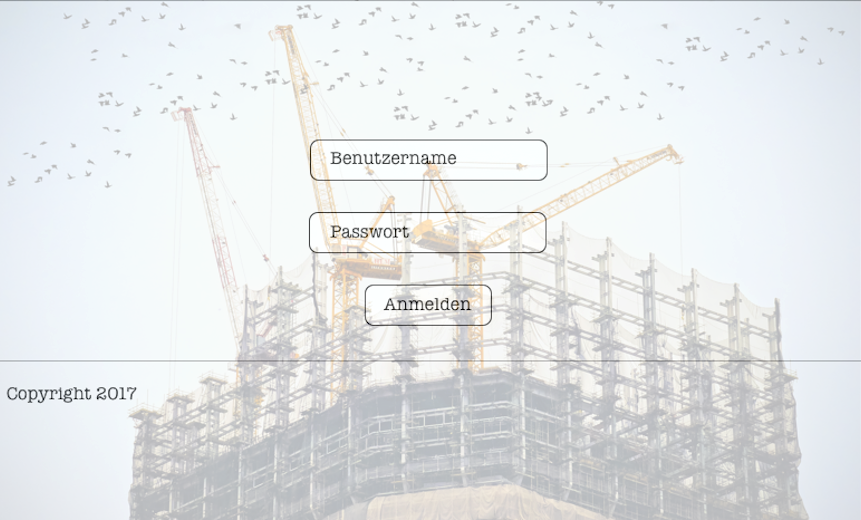
\includegraphics[scale=1]{img/Mockup1Teil1.png}
	\captionof{figure}{\label{abb:mockup1.1}Das erste Mockup}
	\vspace{2em}
\end{minipage}


\begin{minipage}{\linewidth}
	\centering 
	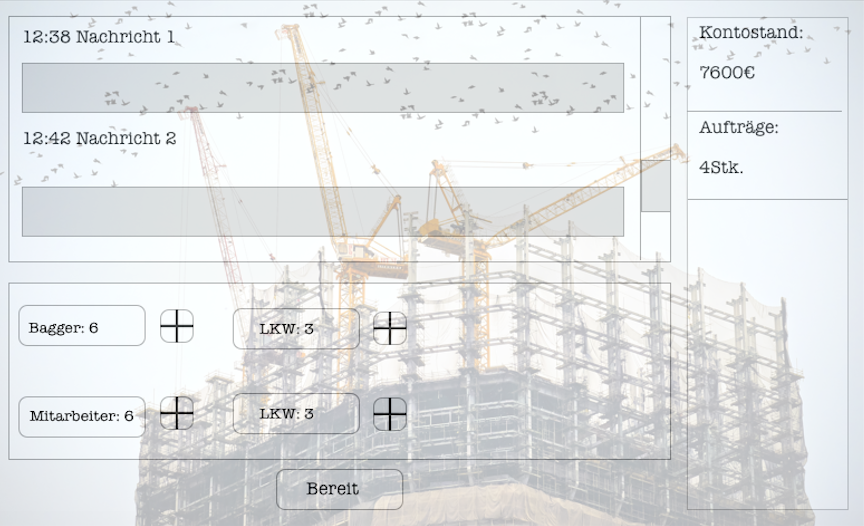
\includegraphics[scale=1]{img/Mockup1Teil2.png}
	\captionof{figure}{\label{abb:mockup1.2}Das erste Mockup}
	\vspace{2em}
\end{minipage}
